\documentclass{article}


\usepackage[english]{babel}
\usepackage[letterpaper,top=2cm,bottom=2cm,left=3cm,right=3cm,marginparwidth=1.75cm]{geometry}
\usepackage{amsmath}
\usepackage{graphicx}
\usepackage[colorlinks=true, allcolors=blue]{hyperref}

\title{Anonymous provision of services via blockchain}
\author{Stanisław Barański}
\date{December 2021}

\providecommand{\keywords}[1]{\textbf{Keywords:} #1}


\begin{document}
\maketitle

\begin{abstract}
Lorem ipsum\ldots
\end{abstract}
\keywords{data privacy, privacy preserving, zk-SNARK, blockchain}



\section{Problem statement}
Service providers (SP) like: lawyers, laboratories, auditors, or banks, to provide services, require data that is often associated with user identity.

Providing personal information exposes users to privacy risk, i.e. potential loss of control over personal information ~\cite{smith2011information}. 

Such user information can be then used deliberately or unintentionally (e.g, by theft) for: insider disclosure, unauthorized access, or commercial gains. For example, by reselling it to marketers, finantial institutions, other businesses, government agencies, or even cybercriminals. Which in turn can lead to profiled advertisements, or cryminal activities like identity theft or illegal tracking and surveillance~\cite{smith2011information}.

The guarantee of the privacy of the data is based on a trust assumptions and security of IT systems. However, most of the service providers don't need the information of user identity for other reasons than payment, communication, or logistics. 

It would be desirable if the user could keep its identity private, while service provider still provide its services. This could lead to reduced trust that users have to put on SP and less responsibility borne by SP.

In this paper we propose a protocol for anonymous provision of services via blockchain and cryptography techniques. Specificaly, we use
\begin{enumerate}
    \item \textbf{confidential blockchain} to process payment for a service without revealing a user's identity.
    \item \textbf{zero-knowledge proofs} — to proof the payment for the service without revealing the payment itself.
    \item \textbf{encryption scheme and blockchain} — to asynchronously deliver the results of the made service back to the user.
\end{enumerate}

\section{State of the art}

Verifiable Document Redacting ~\cite{chabanne2017verifiable} is a protocol for erasing confidential information from authenticated images in verifiable manner. In other words, the protocol allows verifying that only the fields that cover personal information has been blacked out from the authenticated image. This allows users to provide required images without exposing their personal information, and SPs to authenticate the modified images, such that they are sure that only the stated fields have been blacked out and nothing else was touched. 
% In this paper we extend the idea to a whole user-to-service-provider protocol

Authors of the paper~\cite{lin2021efficient} propose a system for Privacy-Preserving Credit Score System. Letting banks to calculate creditworthness without learning user private information like registration, hobbies, credit, relationships, and inquiry. To achieve this they use Paillier encryption and noninteractive zero-Knowledge schemes (NIZK).

\section{Coverage}

Non invasive tests — those which patients can sample themselves: 
\begin{enumerate}
    \item Urine tests
    \item Stool tests
    \item Saliva tests
\end{enumerate}

\section{Solution}


\begin{figure}[htbp]
\centerline{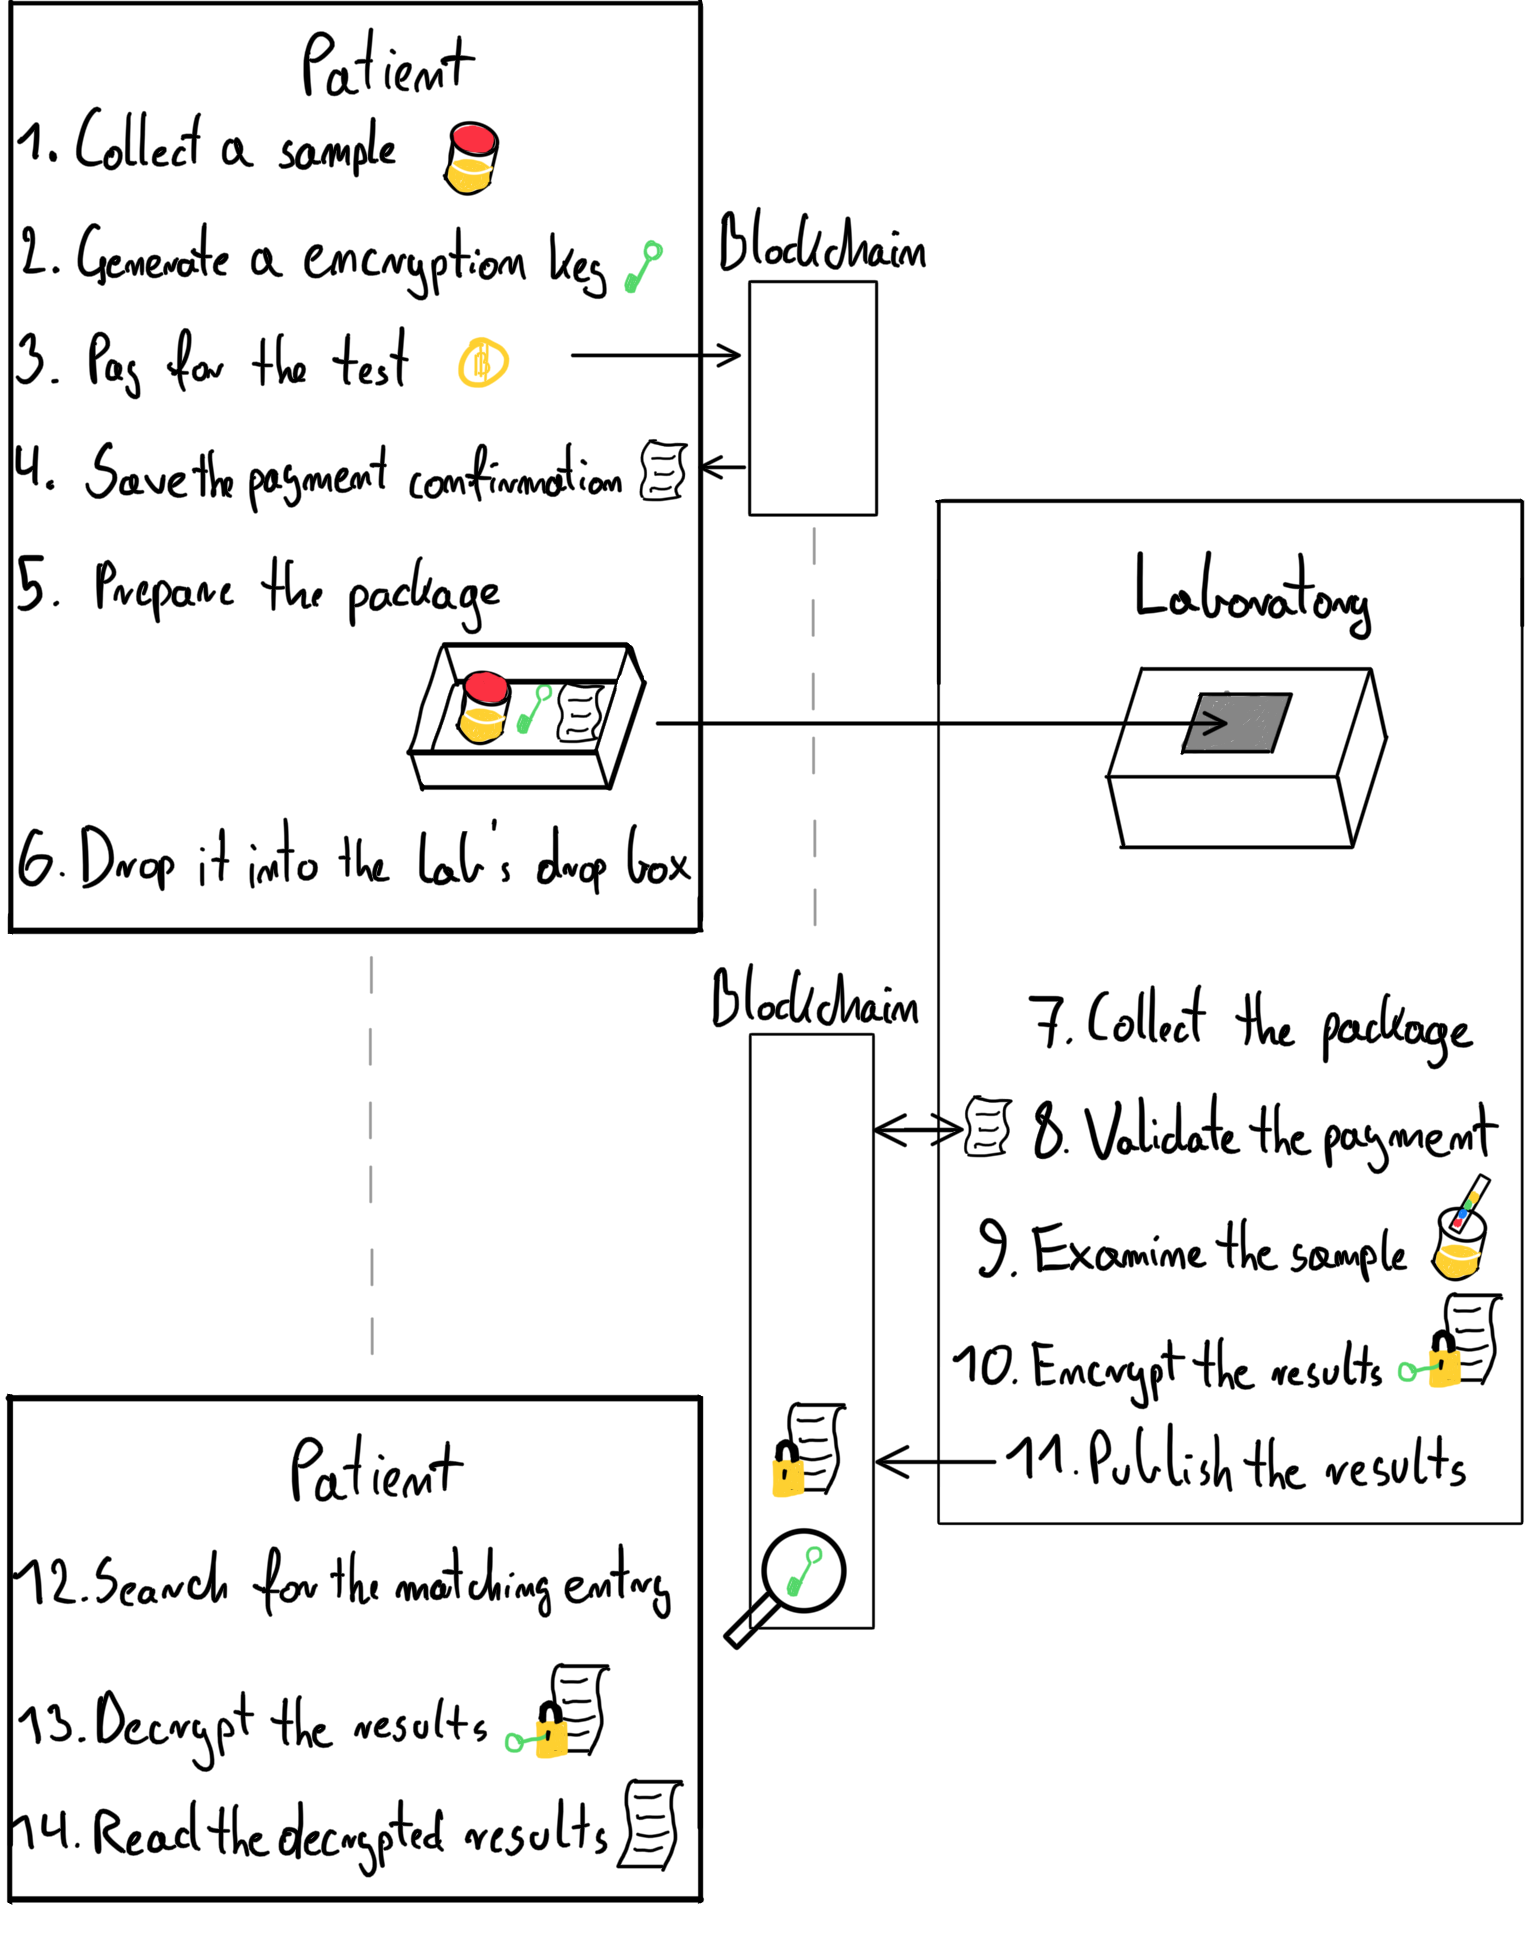
\includegraphics[width=\linewidth]{sequence-flow.png}}
\caption{Sequence flow}
\label{fig:sequence-flow}
\end{figure}



\section{Blockchains}
\paragraph{Monero}
Monero offers out-of-the-box proving/checking confidental transactions. \href{https://www.getmonero.org/resources/user-guides/prove-payment.html}

\paragraph{ZCash}
ZCash offers payment disclosure as a preview feature.
\href{https://garethtdavies.medium.com/an-introduction-to-payment-disclosure-in-zcash-96748c209d49}

\href{https://garethtdavies.medium.com/an-introduction-to-payment-disclosure-in-zcash-96748c209d49}

\section{Applications}
\subsection{Anonymous clinical tests}
Bodybuilders, athletes,  weightlifters, cyclists, football and rugby players have to pass anti-doping tests before attending the competition. 

Patients willing to check steroid tests, drug tests, venereal diseases — anything that they wouldn't want to share with anyone, have to risk that the data stored in laboratory won't get to unauthorized hands like attacker or malicious worker.

Analysis of urine, saliva, stool, or blood. 

\subsection{Anonymous lawyer consultations}

People willing to take business action that may be risky or not yet fully legistlated, may be willing to receive the estimation of risks and repercussions of such action.
Such protocol would provide a mechanism for 


\subsection{Anonymous financial trustworthiness evaluation}

Evaluating financial trustworthiness is required when user want to, for example issue a credit card, take loan for a home, or rent a car. 
As defined in~\cite{lin2021efficient}, such a system consist of three parties: (i) users, (ii) credit bureaus, and (iii) creditors. Users willing to take a credit, have to provide to the credit bureaus, their financial activities like: new account creation, account balance, credit card utilization, credit inquires, and payment history. Such information are then submitted to creditors to compute the user's credit score. 

\subsection{Anonymous physical delivery e-commerce}
% TODO write about
~\cite{birjoveanu2015anonymity}

\bibliographystyle{alpha}
\bibliography{bibliography}

\end{document}
